\documentclass[solution, letterpaper]{cs121}

\usepackage{graphicx}

%% Please fill in your name and collaboration statement here.
%\newcommand{\studentName}{Renzo Lucioni and Daniel Broudy}
%\newcommand{\collaborationStatement}{I collaborated with...}
\newcommand{\solncolor}{red}
\begin{document}

\header{1}{March 5, 2013, at 11:40 AM}{}{}

%%%%%%%%%%%%%%%%%%%%%%%%%%%%%%%%%%%%%%%%%%%%%%%%%%%%
\section{Quantitative Results}
\subsection*{Dimension 0 - Weights Assigned Randomly}

The following is a graph showing the average tree size over 5 trials for several values of $n$: 
\begin{center}
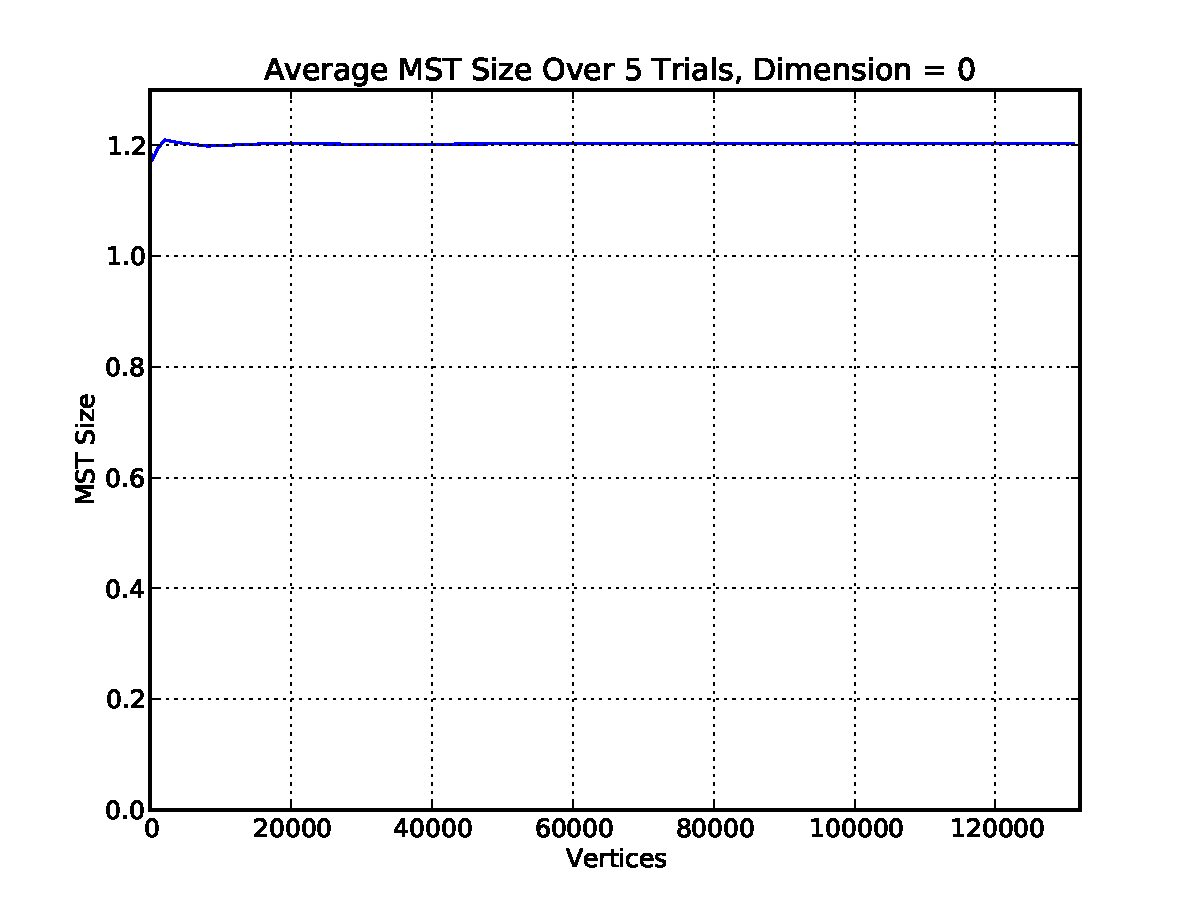
\includegraphics[scale=0.8]{graphs/kruskals-dimension-0.pdf}
\end{center}

A simple function that describes this plot is $f(n) \approx 1.2$

\pagebreak
\subsection*{Dimension 2 - Unit Square}

The following is a graph showing the average tree size over 5 trials for several values of $n$:
\begin{center}
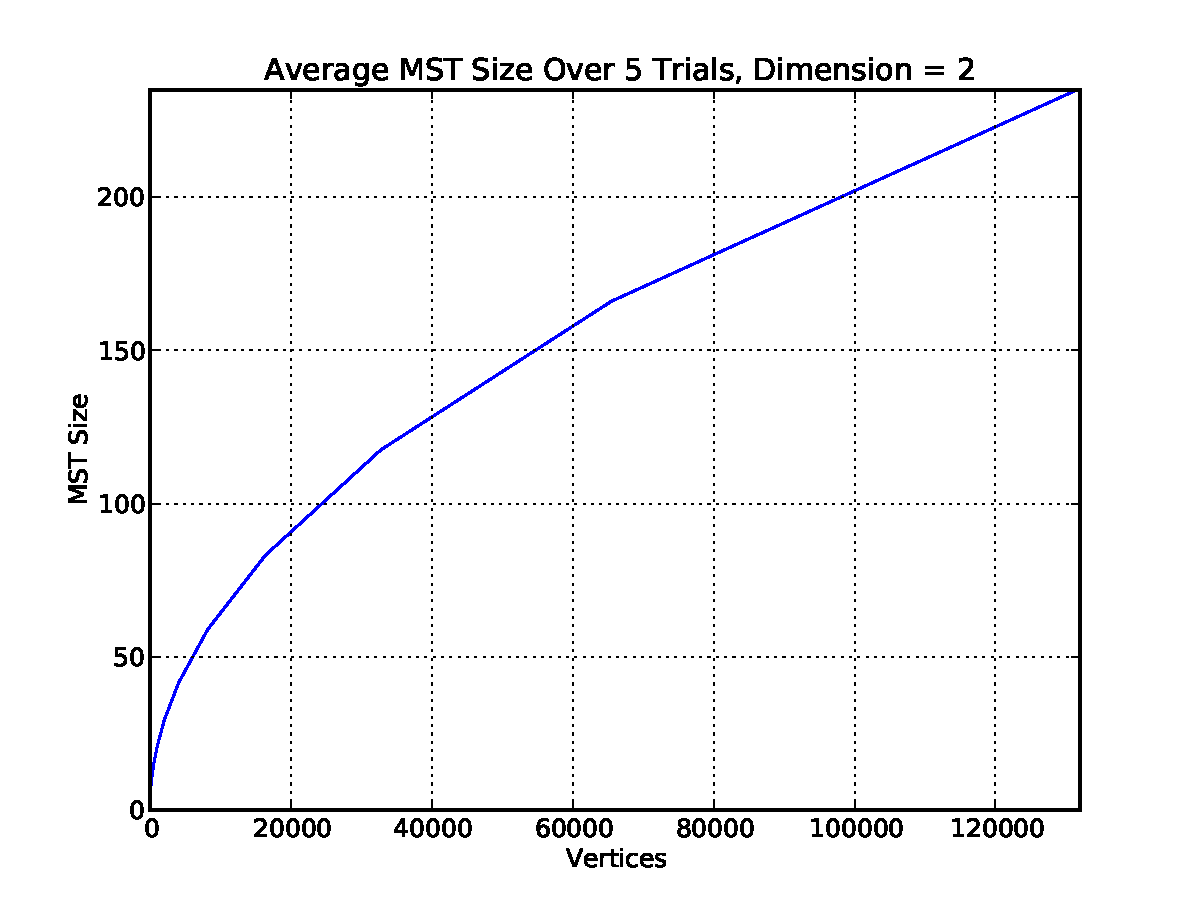
\includegraphics[scale=0.8]{graphs/kruskals-dimension-2.pdf}
\end{center}

Function is of the form $f(n)=an^b$ where $a > 0$ and $\frac{1}{2} \leq b \leq 1$. From mathematica on 2-dimensions we achieved $a=0.647963$ and $b=0.50009$ as the best fit values for this function giving us the following best guess for $f(n)$:
\[f(n) \approx 0.65 n^{\frac{1}{2}}\]

\pagebreak
\subsection*{Dimension 3 - Unit Cube}

The following is a graph showing the average tree size over 5 trials for several values of $n$:
\begin{center}
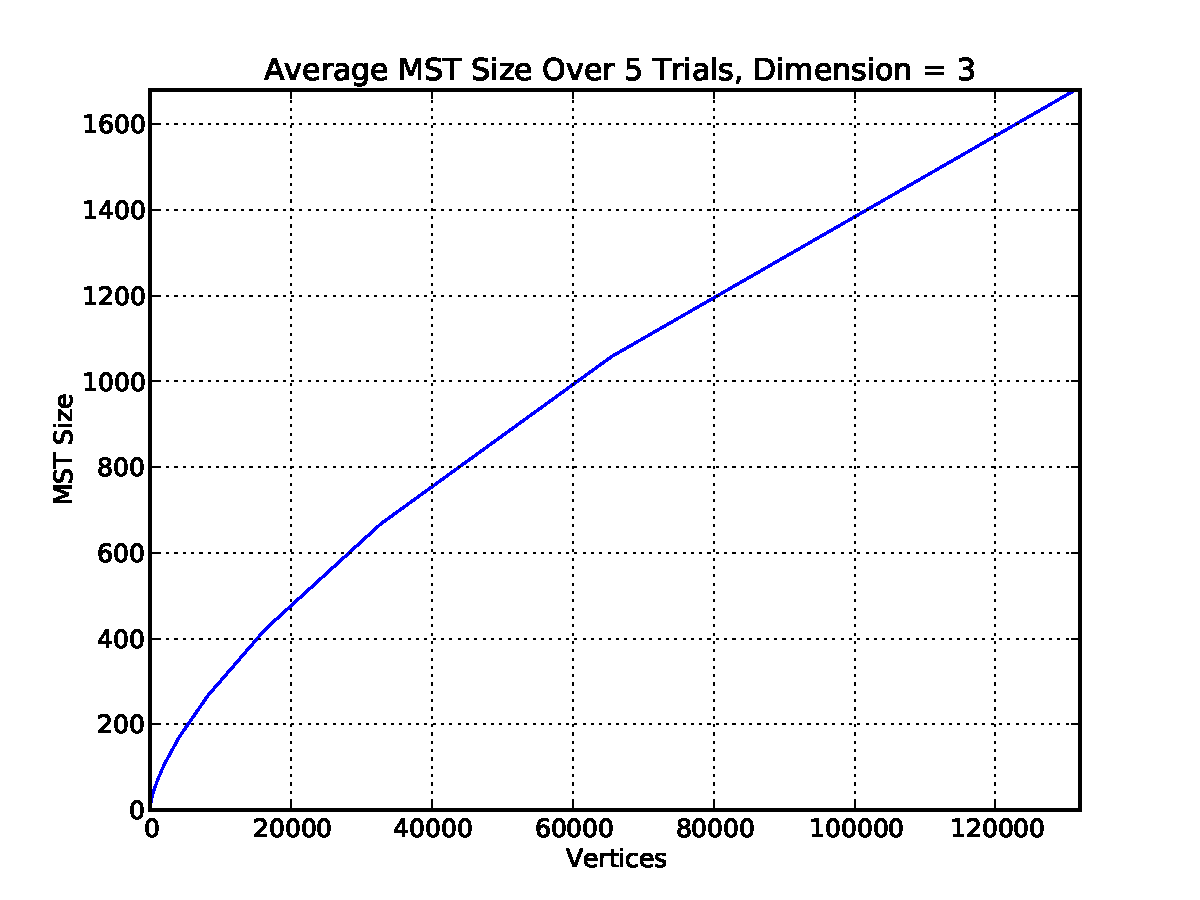
\includegraphics[scale=0.8]{graphs/kruskals-dimension-3.pdf}
\end{center}

Function is of the form $f(n)=an^b$ where $a > 0$ and $\frac{1}{2} \leq b \leq 1$. From mathematica on 2-dimensions we achieved $a=0.68055$ and $b=0.662729$ as the best fit values for this function giving us the following best guess for $f(n)$:
\[f(n) \approx 0.68n^{\frac{2}{3}}\]

\pagebreak
\subsection*{Dimension 4 - Hypercube}

The following is a graph showing the average tree size over 5 trials for several values of $n$:
\begin{center}
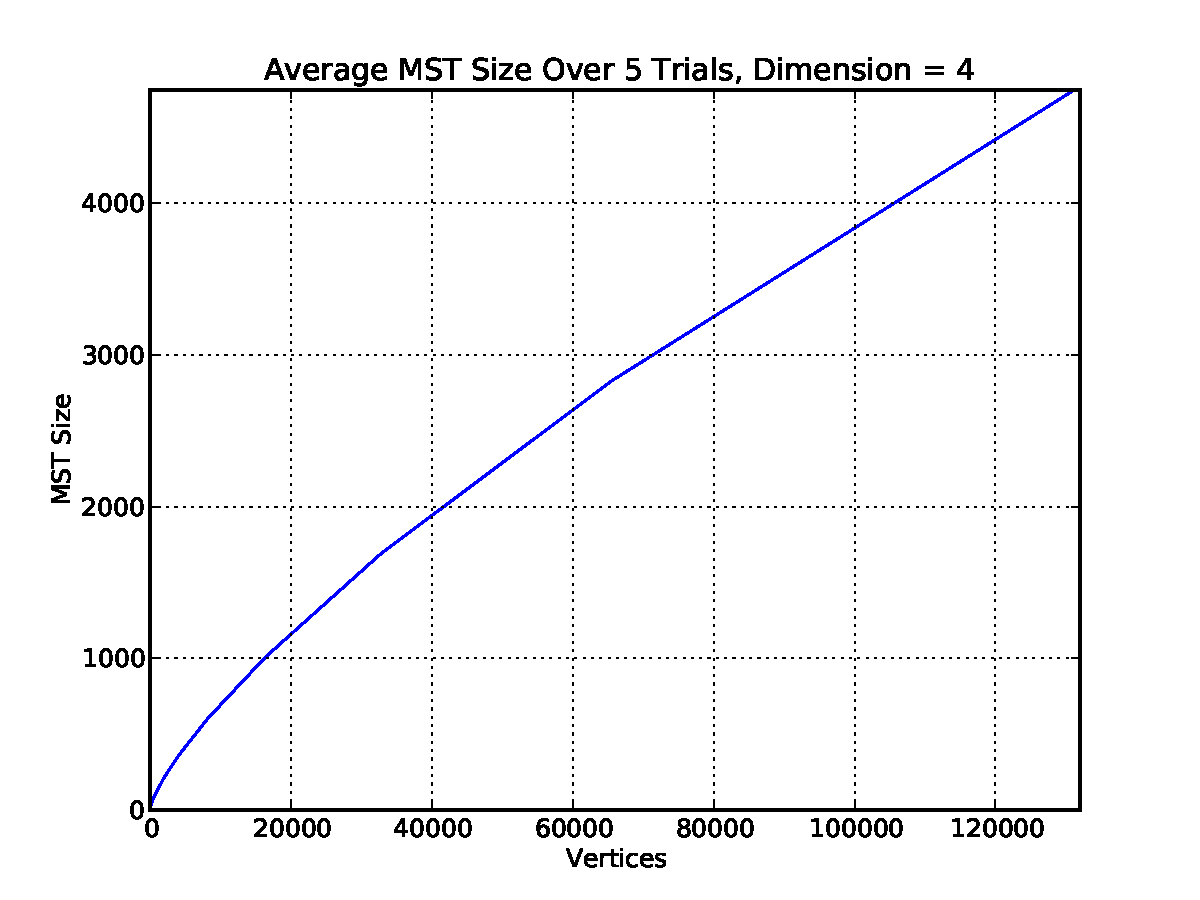
\includegraphics[scale=0.8]{graphs/kruskals-dimension-4.pdf}
\end{center}

Function is of the form $f(n)=an^b$ where $a > 0$ and $\frac{1}{2} \leq b \leq 1$. From mathematica on 2-dimensions we achieved $a=0.744403$ and $b=0.74331$ as the best fit values for this function giving us the following best guess for $f(n)$:
\[f(n) \approx 0.74n^{\frac{3}{4}}\]
\pagebreak
\section*{Discussion}

explain choice of Kruskal's, and our approach to helping the program handle large $n$ (we threw out heavy edges which were unlikely to be included in the MST; we plotted the heaviest edges included in the MSTs for each dimension, then based our limit off of the data we gathered; throwing away edges in this manner will never lead to a situation where the program returns the wrong tree because we are truncating the list that Kruskal's pulls edges from at a point past where the algorithm stops using the array)\\ \\
Are the growth rates (the f(n)) surprising? Can you come up with an explanation for them? \\ \\
How long does it take your algorithm to run? Does this make sense? Do you notice things like the cache size of your computer having an effect? \\ \\
Did you have any interesting experiences with the random number generator? Do you trust it? \\ \\


\end{document}



